\documentclass[a4paper, 14pt]{extarticle}

% Поля
%--------------------------------------
\usepackage{geometry}
\geometry{a4paper,tmargin=2cm,bmargin=2cm,lmargin=3cm,rmargin=1cm}
%--------------------------------------


%Russian-specific packages
%--------------------------------------
\usepackage[T2A]{fontenc}
\usepackage[utf8]{inputenc}
\usepackage[english, main=russian]{babel}
%--------------------------------------

\usepackage{textcomp}

% Красная строка
%--------------------------------------
\usepackage{indentfirst}
%--------------------------------------


%Graphics
%--------------------------------------
\usepackage{graphicx}
\graphicspath{ {./images/} }
\usepackage{wrapfig}
%--------------------------------------

% Полуторный интервал
%--------------------------------------
\linespread{1.3}
%--------------------------------------

%Выравнивание и переносы
%--------------------------------------
% Избавляемся от переполнений
\sloppy
% Запрещаем разрыв страницы после первой строки абзаца
\clubpenalty=10000
% Запрещаем разрыв страницы после последней строки абзаца
\widowpenalty=10000
%--------------------------------------

%Списки
\usepackage{enumitem}

%Подписи
\usepackage{caption}

%Гиперссылки
\usepackage{hyperref}

\hypersetup {
	unicode=true
}

%Рисунки
%--------------------------------------
\DeclareCaptionLabelSeparator*{emdash}{~--- }
\captionsetup[figure]{labelsep=emdash,font=onehalfspacing,position=bottom}
%--------------------------------------

\usepackage{tempora}

%Листинги
%--------------------------------------
\usepackage{listings}
\lstset{
  basicstyle=\ttfamily\footnotesize,
  %basicstyle=\footnotesize\AnkaCoder,        % the size of the fonts that are used for the code
  breakatwhitespace=false,         % sets if automatic breaks shoulbd only happen at whitespace
  breaklines=true,                 % sets automatic line breaking
  captionpos=t,                    % sets the caption-position to bottom
  inputencoding=utf8,
  frame=single,                    % adds a frame around the code
  keepspaces=true,                 % keeps spaces in text, useful for keeping indentation of code (possibly needs columns=flexible)
  keywordstyle=\bf,       % keyword style
  numbers=left,                    % where to put the line-numbers; possible values are (none, left, right)
  numbersep=5pt,                   % how far the line-numbers are from the code
  xleftmargin=25pt,
  xrightmargin=25pt,
  showspaces=false,                % show spaces everywhere adding particular underscores; it overrides 'showstringspaces'
  showstringspaces=false,          % underline spaces within strings only
  showtabs=false,                  % show tabs within strings adding particular underscores
  stepnumber=1,                    % the step between two line-numbers. If it's 1, each line will be numbered
  tabsize=2,                       % sets default tabsize to 8 spaces
  title=\lstname                   % show the filename of files included with \lstinputlisting; also try caption instead of title
}
%--------------------------------------

%%% Математические пакеты %%%
%--------------------------------------
\usepackage{amsthm,amsfonts,amsmath,amssymb,amscd}  % Математические дополнения от AMS
\usepackage{mathtools}                              % Добавляет окружение multlined
\usepackage[perpage]{footmisc}
%--------------------------------------

%--------------------------------------
%			НАЧАЛО ДОКУМЕНТА
%--------------------------------------

\begin{document}

%--------------------------------------
%			ТИТУЛЬНЫЙ ЛИСТ
%--------------------------------------
\begin{titlepage}
\thispagestyle{empty}
\newpage


%Шапка титульного листа
%--------------------------------------
\vspace*{-60pt}
\hspace{-65pt}
\begin{minipage}{0.3\textwidth}
\hspace*{-20pt}\centering

\includegraphics[width=\textwidth]{emblem}
\end{minipage}
\begin{minipage}{0.67\textwidth}\small \textbf{
\vspace*{-0.7ex}
\hspace*{-6pt}\centerline{Министерство науки и высшего образования Российской Федерации}
\vspace*{-0.7ex}
\centerline{Федеральное государственное автономное образовательное учреждение }
\vspace*{-0.7ex}
\centerline{высшего образования}
\vspace*{-0.7ex}
\centerline{<<Московский государственный технический университет}
\vspace*{-0.7ex}
\centerline{имени Н.Э. Баумана}
\vspace*{-0.7ex}
\centerline{(национальный исследовательский университет)>>}
\vspace*{-0.7ex}
\centerline{(МГТУ им. Н.Э. Баумана)}}
\end{minipage}
%--------------------------------------

%Полосы
%--------------------------------------
\vspace{-25pt}
\hspace{-35pt}\rule{\textwidth}{2.3pt}

\vspace*{-20.3pt}
\hspace{-35pt}\rule{\textwidth}{0.4pt}
%--------------------------------------

\vspace{1.5ex}
\hspace{-35pt} \noindent \small ФАКУЛЬТЕТ\hspace{80pt} <<Информатика и системы управления>>

\vspace*{-16pt}
\hspace{47pt}\rule{0.83\textwidth}{0.4pt}

\vspace{0.5ex}
\hspace{-35pt} \noindent \small КАФЕДРА\hspace{50pt} <<Теоретическая информатика и компьютерные технологии>>

\vspace*{-16pt}
\hspace{30pt}\rule{0.866\textwidth}{0.4pt}

\vspace{11em}

\begin{center}
\Large {\bf Лабораторная работа № 5} \\
\large {\bf по курсу <<Численные методы линейной алгебры>>} \\
\large <<Метод Якоби и Зейделя решения СЛАУ>>
\end{center}\normalsize

\vspace{8em}


\begin{flushright}
  {Студент группы ИУ9-72Б Старовойтов А. И. \hspace*{15pt}\\
  \vspace{2ex}
  Преподаватель Посевин Д. П.\hspace*{15pt}}
\end{flushright}

\bigskip

\vfill


\begin{center}
\textsl{Москва 2025}
\end{center}
\end{titlepage}
%--------------------------------------
%		КОНЕЦ ТИТУЛЬНОГО ЛИСТА
%--------------------------------------

\renewcommand{\ttdefault}{pcr}

\setlength{\tabcolsep}{3pt}
\newpage
\setcounter{page}{2}

\section{Задание}\label{Sect::task}

Реализовать итерационные методы Якоби и Зейделя решения СЛАУ. Сравнить
эффективность двух алгоритмов.

\section{Реализация}\label{Sect::impl}

Исходный код программы представлен в листингах~\ref{lst:code1}--~\ref{lst:code2}.

\begin{figure}[!htb]
\begin{lstlisting}[language={},caption={Методы Якоби и Зейделя решения СЛАУ},label={lst:code1}]
using Test
using Random
using LinearAlgebra

Random.seed!(42)

generate_matrix(n) = begin
    A = rand(n, n)
    for i in 1:n
        A[i, i] = sum(abs(A[i, j]) for j in 1:n if j != i) + rand() + 1.0
    end
    return A
end

check_convergence(A) = begin
    for i in axes(A, 1)
        if abs(A[i, i]) <= sum(abs(A[i, j]) for j in axes(A, 2) if j != i)
            return false
        end
    end
    return true
end

yakobi(A, b) = begin
    if !check_convergence(A)
        error("Matrix is not convergent")
    end

    x = zeros(size(A, 1))
    eps = 1e-6
    max_iterations = 10000
    for i in 1:max_iterations
        x_prev = copy(x)
        for j in axes(A, 1)
            x[j] = (b[j] - sum(A[j, k] * x_prev[k] for k in axes(A, 2) if k != j)) / A[j, j]
        end
        if norm(x - x_prev) < eps
            println("Desired accuracy achieved")
            return x, i
        end
    end
    println("Desired accuracy not achieved")
    return x, max_iterations
end

\end{lstlisting}
\end{figure}

% \newpage

\begin{figure}[!htb]
\begin{lstlisting}[language={},caption={Методы Якоби и Зейделя решения СЛАУ (продолжение)},label={lst:code2}]
zeidel(A, b) = begin
    if !check_convergence(A)
        error("Matrix is not convergent")
    end

    x = zeros(size(A, 1))
    eps = 1e-6
    max_iterations = 10000
    for i in 1:max_iterations
        x_prev = copy(x)
        for j in axes(A, 1)
            x[j] = (b[j] - sum(A[j, k] * x[k] for k in axes(A, 2) if k != j)) / A[j, j]
        end
        if norm(x - x_prev) < eps
            println("Desired accuracy achieved")
            return x, i
        end
    end
    println("Desired accuracy not achieved")
    return x, max_iterations
end

@test zeidel([4.0 0.24 -0.08; 0.09 3.0 -0.15; 0.04 -0.08 4.0], [8.0, 9.0, 20.0])[1] == [1.909, 3.195, 5.045] atol=1e-3
@test yakobi([4.0 0.24 -0.08; 0.09 3.0 -0.15; 0.04 -0.08 4.0], [8.0, 9.0, 20.0])[1] == [1.909, 3.195, 5.045] atol=1e-3

main() = begin
    A = generate_matrix(500)
    b = rand(500)

    time_zeidel = @elapsed begin
        x, iterations = zeidel(A, b)
    end
    println("Zeidel:")
    println("Iterations: ", iterations)
    println("Time: ", time_zeidel * 1000, " ms")
    println("Error: ", norm(A * x - b))

    time_yakobi = @elapsed begin
        x, iterations = yakobi(A, b)
    end
    println("Yakobi:")
    println("Iterations: ", iterations)
    println("Time: ", time_yakobi * 1000, " ms")
    println("Error: ", norm(A * x - b))
end

main()
\end{lstlisting}
\end{figure}

\clearpage
\section{Результаты}\label{Sect::res}

Результат запуска представлен на рисунке~\ref{fig:img1}.

\begin{figure}[!htb]
	\centering
	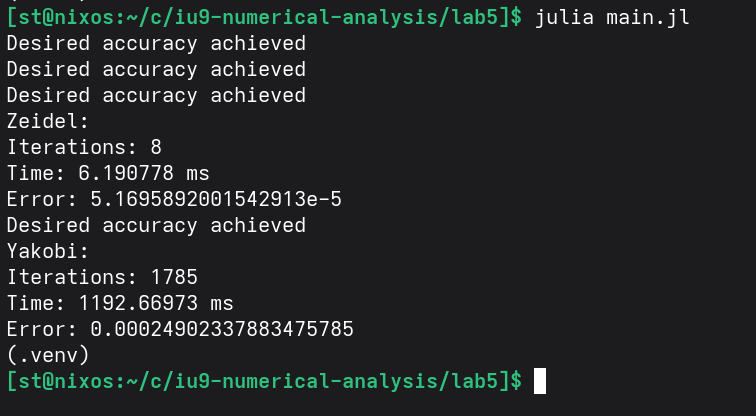
\includegraphics[width=0.8\textwidth]{img1}
\caption{Результат}
\label{fig:img1}
\end{figure}

\clearpage
\section{Выводы}\label{Sect::fin}

Результатом выполнения данной лабораторной работы является реализация
алгоритмов, позволяющих решать системы линейных алгебраических уравнений, а
также измерение и сравнение их эффективности.

\end{document}
